\documentclass{article}




\usepackage{fullpage}
\usepackage{nopageno}
\usepackage{amsmath}
\usepackage{amsfonts}
\usepackage{graphicx}
\usepackage{framed}
\usepackage{algorithmic}
\usepackage{xcolor}

\definecolor{dark_red}{rgb}{0.5,0.0,0.0}
\definecolor{dark_green}{rgb}{0.0,0.5,0.0}
\definecolor{dark_blue}{rgb}{0.0,0.0,0.5}
\definecolor{blue}{rgb}{0.0,0.0,1.0}

\newcommand{\dr}[1]{\textcolor{dark_red}{#1}}
\newcommand{\dg}[1]{\textcolor{dark_green}{#1}}
\newcommand{\db}[1]{\textcolor{dark_blue}{#1}}
\newcommand{\blue}[1]{\textcolor{blue}{#1}}



\usepackage{fancyhdr}
%\setlength{\footheight}{15.2pt}
\pagestyle{fancy}
\fancyhead[C]{Wentworth Institute of Technology, MATH2025}
\fancyfoot[C]{Author: Shawn Eastwood}
\renewcommand{\headsep}{25pt}
\renewcommand{\headrulewidth}{1pt}
\renewcommand{\footrulewidth}{1pt}




\begin{document}


\section*{Polar Coordinates}

\begin{tabular}{cc}
\parbox{0.5\textwidth}{
As an alternative to Cartesian coordinates, polar coordinates provide another means of quantifying the position of a point using two numbers. Polar coordinates describe a point \(P\)'s location using a pair of numbers \((r, \theta)\) instead of \((x, y)\). \(r\) denotes the ``distance" of \(P\) from the origin, while \(\theta\) denotes the counterclockwise rotation from the positive \(x\)-axis required to aim at point \(P\). Polar coordinates are illustrated by the image on the right.
\begin{itemize}
\item \(\theta\) will always be measured in radians. 
\item The rotation \(\theta\) is always measured relative to the positive \(x\)-axis.
\item A clockwise rotation corresponds to a negative value of \(\theta\).
\end{itemize} 
} & \parbox{0.5\textwidth}{
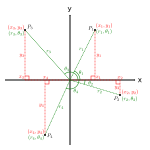
\includegraphics[width = 0.5\textwidth]{cartesian_vs_polar_coordinates}
}
\end{tabular}

\begin{tabular}{cc}
\parbox{0.5\textwidth}{
Despite \(r\) denoting the ``distance" required to reach point \(P\), \(r\) can still be negative. Initially facing in the direction of the positive \(x\)-axis, coordinate \(\theta\) denotes the counterclockwise rotation required to lineup point \(P\). \(r\) is positive if forwards movement is necessary to reach point \(P\), while \(r\) is {\bf negative} if {\bf backwards} movement is required to reach point \(P\).
} & \parbox{0.5\textwidth}{
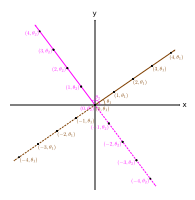
\includegraphics[width = 0.5\textwidth]{negative_r}
}
\end{tabular}


Given polar coordinate \((r, \theta)\), for every integer \(k \in \mathbb{Z}\), the polar coordinates \((r, \theta + k \cdot 2\pi) = (r, \theta + 2 k \pi)\) and \((-r, \theta + \pi + k \cdot 2\pi) = (-r, \theta + (2k + 1)\pi)\) describe the same point \((r, \theta)\). Adding or subtracting full revolutions from \(\theta\) does not change the referenced point. In addition, adding or subtracting a half revolution followed by sign change of \(r\) does not change the referenced point.

In polar coordinates, 
\[\cdots = (-r, \theta - 3\pi) = (r, \theta - 2\pi) = (-r, \theta - \pi) = (r, \theta) = (-r, \theta + \pi) = (r, \theta + 2\pi) = (-r, \theta + 3\pi) = \cdots\]
all denote the same point. 

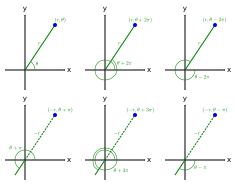
\includegraphics[scale = 0.65]{multiple_polar_coordinates}

\textbf{Examples:}
\begin{itemize}
\item The polar coordinates \((3, 3\pi/4)\), \((3, 11\pi/4)\), \((3, -5\pi/4)\), \((-3, 7\pi/4)\), \((-3, 15\pi/4)\), and \((-3, -\pi/4)\) all describe the same point.
\end{itemize}



\subsection*{Polar coordinates and the trigonometric ratios}

In the image below, the red unit circle, the green tangent line defined by \(x = 1\), and the blue tangent line defined by \(y = 1\) are shown. Starting from the positive \(x\) axis, rotate by a counterclockwise angle of \(\theta\). A ray projected forwards corresponds to positive values of \(r\). A ray projected backwards corresponds to negative values of \(r\). The positive ray intersects the unit circle at the point with Cartesian coordinates \((\cos\theta, \sin\theta)\), which also has the polar coordinates \((1, \theta)\). The rays intersect the green tangent line at the point with Cartesian coordinates \((1, \tan\theta)\), which also has the polar coordinates \((\sec\theta, \theta)\). The rays intersect the blue tangent line at the point with Cartesian coordinates \((\cot\theta, 1)\), which also has the polar coordinates \((\csc\theta, \theta)\). These points are depicted in the image below for two different values of \(\theta\), namely \(\theta_1\) and \(\theta_2\). \(\theta_1\) is chosen from the interval \((0,\pi/2)\) and generates the brown rays, while \(\theta_2\) is chosen from the interval \((\pi/2,\pi)\) and generates the pink rays.

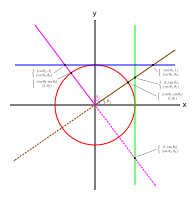
\includegraphics[scale = 0.9]{the_unit_circle_and_polar_coordinates}




\subsection*{Polar to Cartesian conversion}

\begin{tabular}{cc}
\parbox{0.5\textwidth}{
Given an arbitrary polar coordinate \((r, \theta)\), there is only one Cartesian coordinate \((x, y)\) for the point generated by \((r, \theta)\). Project the ray rotated a counterclockwise angle of \(\theta\) from the positive \(x\)-axis. This ray intersects the unit circle at a point with Cartesian coordinates \((\cos\theta, \sin\theta)\) and polar coordinates \((1, \theta)\). Scaling every length uniformly by \(r\) changes the Cartesian coordinate to \((r\cos\theta, r\sin\theta)\) and the polar coordinate to \((r, \theta)\). Therefore:
\[\left\{\begin{array}{c} x = r\cos\theta \\ y = r\sin\theta \end{array}\right.\]
is how the polar coordinate \((r, \theta)\) is converted to Cartesian coordinate \((x, y)\).
} & \parbox{0.5\textwidth}{
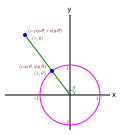
\includegraphics[width = 0.5\textwidth]{polar_to_cartesian_conversion}
}
\end{tabular}

\textbf{Examples:}
\begin{itemize}
\item The polar coordinate \((r, \theta) = (3, \pi/5)\) converted to a Cartesian coordinate is \((x, y) = (3\cos(\pi/5), 3\sin(\pi/5)) \approx (2.42705, 1.76336)\)
\item The polar coordinate \((r, \theta) = (7, 0.77\pi)\) converted to a Cartesian coordinate is \((x, y) = (7\cos(0.77\pi), 7\sin(0.77\pi)) \approx (-5.25078, 4.62918)\)
\item The polar coordinate \((r, \theta) = (2.6, -1.67\pi)\) converted to a Cartesian coordinate is \\ \((x, y) = (2.6\cos(-1.67\pi), 2.6\sin(-1.67\pi)) \approx (1.32351, 2.23793)\)
\item The polar coordinate \((r, \theta) = (2.6, 0.33\pi)\) converted to a Cartesian coordinate is \\ \((x, y) = (2.6\cos(0.33\pi), 2.6\sin(0.33\pi)) \approx (1.32351, 2.23793)\)
\item The polar coordinate \((r, \theta) = (-3, \pi/5)\) converted to a Cartesian coordinate is \((x, y) = (-3\cos(\pi/5), -3\sin(\pi/5)) \approx (-2.42705, -1.76336)\)
\end{itemize}




\subsection*{Cartesian to polar conversion}

Given an arbitrary Cartesian coordinate \((x, y)\), a polar coordinate \((r, \theta)\) that generates the same point as \((x, y)\) is sought.

There are infinitely many choices of polar coordinate \((r,\theta)\) for the given Cartesian coordinate \((x,y)\). To limit our choices down to one alternative, the following restrictions will be placed on \(r\) and \(\theta\):
\[\left\{\begin{array}{c} r \geq 0 \\ (r = 0) \implies (\theta = 0) \\ -\pi < \theta \leq \pi \end{array}\right.\] 
\begin{itemize}
\item Since \(r \geq 0\), only non-negative choices of \(r\) will be considered, so \(r\) is simply the distance that the point \((x,y)\) is from the origin: \(r = \sqrt{x^2 + y^2}\). 
\item The condition \((r = 0) \implies (\theta = 0)\) means that \(\theta = 0\) if \(r = 0\), which means that the \(\theta\) coordinate of the origin point, which could have been any value, is defaulted to \(\theta = 0\). 
\item The condition \(-\pi < \theta \leq \pi\) means that a counterclockwise twist is used to reach points above the \(x\)-axis, and a clockwise twist is used to reach points beneath the \(x\)-axis. Moreover, a twist of \(\pi\) (which is counterclockwise) is used to reach the negative \(x\)-axis.
\end{itemize}

It is clear that \(r\) is simply the distance that the point \((x,y)\) is from the origin: \(r = \sqrt{x^2 + y^2}\). Computing \(\theta\) is a more difficult task. 

To find \(\theta\), consider the line segment that connects the origin to point \((x, y)\). The counterclockwise angle that this line segment makes with the positive \(x\)-axis is \(\theta\). Extrapolating this line segment to a line, this line will intersect the vertical line defined by \(x = 1\) at the Cartesian point \((1, y/x)\). This is because the line segment has a slope of \(y/x\), so the change in \(y\) over a unit change in \(x\) is \(y/x\). {\bf Use the image below for illustration.} Given a line that makes a counterclockwise angle of \(\theta\) with the \(x\)-axis, this line intersects the line \(x = 1\) at the Cartesian point \((1, \tan\theta)\) (revisit the discussions related to the unit circle). Since \((1, y/x)\) and \((1, \tan\theta)\) are the same point, \(\tan\theta = y/x\). 

The fact that \(\tan\theta = y/x\) can also be established from \(x = r\cos\theta\) and \(y = r\sin\theta\):
\[\frac{y}{x} = \frac{r\sin\theta}{r\cos\theta} = \frac{\sin\theta}{\cos\theta} = \tan\theta\]

In the image below, it can be seen that if \(x > 0\), then \(\theta = \tan^{-1}(y/x)\), whereas if \(x < 0\), then a half rotation needs to be either added to or subtracted from \(\tan^{-1}(y/x)\) to get \(\theta\). 

In the case where \(x < 0\), 
\begin{itemize}
\item If \(y/x \leq 0\), then the range of values of \(\tan^{-1}(y/x)\) is \((-\pi/2, 0]\), so a half rotation must be added to give values of \(\theta\) from the range \((\pi/2, \pi]\) which is a valid subset of the target range \((-\pi, \pi]\). This can be seen with point \((x_3, y_3)\) in the image, where a half rotation needs to be added to \(\tan^{-1}(y_3/x_3)\) to get \(\theta_3\).
\item If \(y/x > 0\), then the range of values of \(\tan^{-1}(y/x)\) is \((0, \pi/2)\), so a half rotation must be subtracted to give values of \(\theta\) from the range \((-\pi, -\pi/2)\) which is a valid subset of the target range \((-\pi, \pi]\). This can be seen with point \((x_4, y_4)\) in the image, where a half rotation needs to be subtracted from \(\tan^{-1}(y_4/x_4)\) to get \(\theta_4\).
\end{itemize}

In summary, 
\begin{itemize}
\item If \(x > 0\), then \(\theta = \tan^{-1}(y/x)\)
\item If \(x = 0\), then
	\begin{itemize}
	\item[*] If \(y > 0\), then \(\theta = \pi/2\)
	\item[*] If \(y = 0\), then \(\theta = 0\) (this is the origin point)
	\item[*] If \(y < 0\), then \(\theta = -\pi/2\)
	\end{itemize}
\item If \(x < 0\), then
	\begin{itemize}
	\item[*] If \(y \geq 0\), then \(\theta = \tan^{-1}(y/x) + \pi\)
	\item[*] If \(y < 0\), then \(\theta = \tan^{-1}(y/x) - \pi\)
	\end{itemize}
\end{itemize}

%From the information \(\tan\theta = y/x\), there are an infinite number of values for \(\theta\) that satisfy this equation. Restricting \(\theta\) to the interval \((-\pi, \pi]\) narrows the possible solutions down to 2 alternatives. When \(y/x > 0\), the candidate values of \(\theta\) are \(\tan^{-1}(y/x)\)

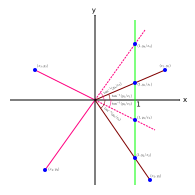
\includegraphics[scale = 0.9]{computing_theta}


\textbf{Examples:}
\begin{itemize}
\item The Cartesian coordinate \((x, y) = (1, 2)\) converted to a polar coordinate gives \(r = \sqrt{1^2 + 2^2} \approx 2.23607\) and \(\theta = \tan^{-1}(2/1) \approx 1.10715\). Hence \((r, \theta) \approx (2.23607, 1.10715)\) is one possible choice of polar coordinate. 
\item The Cartesian coordinate \((x, y) = (4, -3)\) converted to a polar coordinate gives \(r = \sqrt{4^2 + (-3)^2} = 5\) and \(\theta = \tan^{-1}((-3)/4) \approx -0.643501\). Hence \((r, \theta) \approx (5, -0.643501)\) is one possible choice of polar coordinate. 
\item The Cartesian coordinate \((x, y) = (0, 6)\) converted to a polar coordinate gives \(r = \sqrt{0^2 + 6^2} = 6\) and \(\theta = \pi/2 \approx 1.57080\). Hence \((r, \theta) \approx (6, 1.57080)\) is one possible choice of polar coordinate.  
\item The Cartesian coordinate \((x, y) = (0, 0)\) converted to a polar coordinate gives \(r = \sqrt{0^2 + 0^2} = 0\) and \(\theta = 0\). Hence \((r, \theta) = (0, 0)\) is one possible choice of polar coordinate.
\item The Cartesian coordinate \((x, y) = (0, -3)\) converted to a polar coordinate gives \(r = \sqrt{0^2 + (-3)^2} = 3\) and \(\theta = -\pi/2 \approx -1.57080\). Hence \((r, \theta) \approx (3, -1.57080)\) is one possible choice of polar coordinate.
\item The Cartesian coordinate \((x, y) = (-2, 5)\) converted to a polar coordinate gives \(r = \sqrt{(-2)^2 + 5^2} \approx 5.38516\) and \(\theta = \tan^{-1}(5/(-2)) + \pi \approx 1.95130\). Hence \((r, \theta) \approx (5.38516, 1.95130)\) is one possible choice of polar coordinate. 
\item The Cartesian coordinate \((x, y) = (-3, -1)\) converted to a polar coordinate gives \(r = \sqrt{(-3)^2 + (-1)^2} \approx 3.16228\) and \(\theta = \tan^{-1}((-1)/(-3)) - \pi \approx -2.81984\). Hence \((r, \theta) \approx (3.16228, -2.81984)\) is one possible choice of polar coordinate. 
\end{itemize}




\section*{Double Integrals using Polar Coordinates}

\begin{tabular}{cc}
\parbox{0.5\textwidth}{
2D regions in polar coordinates can be quantified by first establishing bounds on \(\theta\), and then establishing bounds on \(r\) that are functions of \(\theta\). In the image to the right, the bounds on \(\theta\) are \(a\) and \(b\): \(a \leq \theta \leq b\). The bounds on \(r\) are functions of \(\theta\): \(h_L(\theta) \leq r \leq h_U(\theta)\). The region itself is:

\[R = \{(r, \theta) | a \leq \theta \leq b \;\&\; h_L(\theta) \leq r \leq h_U(\theta)\}\]

{\bf It will now always be assumed that \(r \geq 0\) for all valid polar regions.}

} & \parbox{0.5\textwidth}{
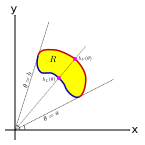
\includegraphics[width = 0.5\textwidth]{general_Polar_region}
}
\end{tabular}

The double integral \(\iint_R f(r,\theta)dA\) over a polar region: 
\[R = \{(r, \theta) | a \leq \theta \leq b \;\&\; h_L(\theta) \leq r \leq h_U(\theta)\}\]
will now be evaluated using nested single variable integrals. To establish the single integral expression for \(\iint_R f(r,\theta)dA\), region \(R\) will be decomposed into a series of \(N\) thin wedges where \(N\) is a large number, as depicted in the image below. For each \(i = 1, 2, ..., N\), the angle of the \(i^{\text{th}}\) wedge is \(\Delta \theta_i\), and \(\theta_i^*\) is a ``representative" \(\theta\) value from the \(i^{\text{th}}\) wedge. Now for each wedge, further partition the wedge into a series of \(M\) ``polar rectangles" where \(M\) is a large number, as depicted in the image below. For each \(i = 1, 2, ..., N\) and for each \(j = 1, 2, ..., M\), the radial thickness of the \(j^{\text{th}}\) polar rectangle in the \(i^{\text{th}}\) wedge is \(\Delta r_{(i,j)}\), and \(r_{(i,j)}^*\) is a ``representative" \(r\) value from the \(j^{\text{th}}\) polar rectangle in the \(i^{\text{th}}\) wedge. 

\begin{center}
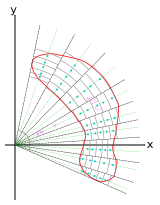
\includegraphics[width = 0.75\textwidth]{polar_riemann_sum}
\end{center}

\begin{tabular}{cc}
\parbox{0.5\textwidth}{
The area of the \(j^{\text{th}}\) polar rectangle in the \(i^{\text{th}}\) wedge is not \(\Delta r_{(i,j)} \Delta\theta_i\). 

To the right is shown a polar rectangle with an angular length of \(\Delta\theta\) and a radial thickness of \(\Delta r\). The average of the inner and outer radii is \(r^*\). It can be computed that the area on this polar rectangle is \((r\Delta\theta)\Delta r = r \Delta r \Delta\theta\).

The area of the \(j^{\text{th}}\) polar rectangle in the \(i^{\text{th}}\) wedge is in fact:
\[\Delta A_{(i,j)} = r_{(i,j)}^* \Delta r_{(i,j)} \Delta \theta_i\]
where an additional factor of \(r_{(i,j)}^*\) has been introduced.
} & \parbox{0.5\textwidth}{

\includegraphics[width = 0.5\textwidth]{polar_rectangle}
}
\end{tabular}

Evaluating the Riemann sum gives:
\begin{align*}
\iint_R f(r,\theta)dA = & \lim_{N \rightarrow +\infty} \lim_{M \rightarrow +\infty} \sum_{i = 1}^N \sum_{j = 1}^M f(r_{(i,j)}^*, \theta_i^*)\Delta A_{(i,j)}
= \lim_{N \rightarrow +\infty} \lim_{M \rightarrow +\infty} \sum_{i = 1}^N \sum_{j = 1}^M f(r_{(i,j)}^*, \theta_i^*)(r_{(i,j)}^* \Delta r_{(i,j)} \Delta\theta_i) \\
= & \lim_{N \rightarrow +\infty} \sum_{i = 1}^N \left(\lim_{M \rightarrow +\infty} \sum_{j = 1}^M f(r_{(i,j)}^*, \theta_i^*) \cdot r_{(i,j)}^* \cdot \Delta r_{(i,j)}\right) \Delta\theta_i \\
= & \lim_{N \rightarrow +\infty} \sum_{i = 1}^N \left(\int_{r = h_L(\theta_i^*)}^{h_U(\theta_i^*)} f(r, \theta_i^*) \cdot r \cdot dr\right) \Delta\theta_i 
= \int_{\theta = a}^b \left(\int_{r = h_L(\theta)}^{h_U(\theta)} f(r, \theta) \cdot r \cdot dr\right) d\theta 
\end{align*}

Therefore:
\[\iint_R f(r,\theta) = \int_{\theta = a}^b \left(\int_{r = h_L(\theta)}^{h_U(\theta)} f(r, \theta) \cdot r \cdot dr\right) d\theta\]
Note the introduction of an additional factor of \(r\) to the integrand when the double integral is replaced with the nested integral.



\vspace{5mm}

\textbf{Example 1:}

\begin{tabular}{cc}
\parbox{0.5\textwidth}{
Consider the polar region:
\[R = \left\{(r, \theta) \middle| \frac{\pi}{4} \leq \theta \leq \frac{5\pi}{4} \;\&\; 2 \leq r \leq 3 \right\}\]
which is depicted on the right. 

Given an arbitrary integrand \(f(r,\theta)\), the double integral over the region \(R\) is: 
\[\iint_R f(r,\theta)dA = \int_{\theta = \pi/4}^{5\pi/4} \left(\int_{r = 2}^3 f(r, \theta) \cdot r \cdot dr\right)d\theta\]
Note the introduction of an additional factor of \(r\) to the integrand when the double integral is replaced with the nested integral.
} & \parbox{0.5\textwidth}{

\includegraphics[width = 0.5\textwidth]{Polar_region_1}
}
\end{tabular}

Consider the specific integrand \(f(r,\theta) = \frac{1}{r}\cos^2\theta\sin^2\theta\). The double integral over \(R\) is:

\begin{align*}
& \iint_R \frac{1}{r}\cos^2\theta\sin^2\theta \cdot dA
= \int_{\theta = \pi/4}^{5\pi/4} \left(\int_{r = 2}^3 \frac{1}{r}\cos^2\theta\sin^2\theta \cdot r \cdot dr\right)d\theta  
= \int_{\theta = \pi/4}^{5\pi/4} \left(\int_{r = 2}^3 \cos^2\theta\sin^2\theta \cdot dr\right)d\theta \\
& = \int_{\theta = \pi/4}^{5\pi/4} r\cos^2\theta\sin^2\theta\Big|_{r = 2}^3 d\theta 
= \int_{\theta = \pi/4}^{5\pi/4} \cos^2\theta\sin^2\theta d\theta 
= \int_{\theta = \pi/4}^{5\pi/4} \left(\frac{1 + \cos(2\theta)}{2}\right)\left(\frac{1 - \cos(2\theta)}{2}\right) d\theta \\ 
& = \int_{\theta = \pi/4}^{5\pi/4} \frac{1 - \cos^2(2\theta)}{4} d\theta 
= \int_{\theta = \pi/4}^{5\pi/4} \frac{1 - \frac{1 + \cos(4\theta)}{2}}{4} d\theta  
= \int_{\theta = \pi/4}^{5\pi/4} \frac{1 - \cos(4\theta)}{8} d\theta  
= \frac{\theta - \frac{1}{4}\sin(4\theta)}{8}\Big|_{\theta = \pi/4}^{5\pi/4} \\  
& = \frac{4\theta - \sin(4\theta)}{32}\Big|_{\theta = \pi/4}^{5\pi/4} 
= \frac{5\pi - \sin(5\pi)}{32} - \frac{\pi - \sin(\pi)}{32}     
= \frac{5\pi}{32} - \frac{\pi}{32} 
= \frac{4\pi}{32}
= \frac{\pi}{8}
\end{align*}




\vspace{5mm}

\textbf{Example 2:}

\begin{tabular}{cc}
\parbox{0.5\textwidth}{
Consider the polar region:
\[R = \left\{(r, \theta) \middle| 0 \leq \theta \leq \frac{\pi}{2} \;\&\; 0 \leq r \leq \sin(2\theta) \right\}\]
which is depicted on the right. 

Given an arbitrary integrand \(f(r,\theta)\), the double integral over the region \(R\) is: 
\[\iint_R f(r,\theta)dA = \int_{\theta = 0}^{\pi/2} \left(\int_{r = 0}^{\sin(2\theta)} f(r, \theta) \cdot r \cdot dr\right)d\theta\]
Note the introduction of an additional factor of \(r\) to the integrand when the double integral is replaced with the nested integral.
} & \parbox{0.5\textwidth}{

\includegraphics[width = 0.5\textwidth]{Polar_region_2}
}
\end{tabular}

Consider the specific integrand \(f(r,\theta) = r\). The double integral over \(R\) is:

\begin{align*} 
& \iint_R r dA 
= \int_{\theta = 0}^{\pi/2} \left(\int_{r = 0}^{\sin(2\theta)} r \cdot r \cdot dr\right)d\theta  
= \int_{\theta = 0}^{\pi/2} \left(\int_{r = 0}^{\sin(2\theta)} r^2 \cdot dr\right)d\theta 
= \int_{\theta = 0}^{\pi/2} \frac{1}{3}r^3 \Big|_{r = 0}^{\sin(2\theta)} d\theta \\
& = \int_{\theta = 0}^{\pi/2} \frac{1}{3}\sin^3(2\theta) d\theta 
= \int_{\theta = 0}^{\pi/2} \frac{1}{3}\sin(2\theta) \cdot \sin^2(2\theta) d\theta 
= \int_{\theta = 0}^{\pi/2} \frac{1}{3}\sin(2\theta)(1 - \cos^2(2\theta)) d\theta \\
& = \int_{\theta = 0}^{\pi/2} -\frac{1}{6}(1 - \cos^2(2\theta)) (-2\sin(2\theta)d\theta) 
= -\frac{1}{6}(\cos(2\theta) - \frac{1}{3}\cos^3(2\theta))\Big|_{\theta = 0}^{\pi/2} \\
& = (-\frac{1}{6}(\cos(\pi) - \frac{1}{3}\cos^3(\pi))) - (-\frac{1}{6}(\cos(0) - \frac{1}{3}\cos^3(0))) 
= (-\frac{1}{6}(-1 + \frac{1}{3})) - (-\frac{1}{6}(1 - \frac{1}{3})) \\
& = (\frac{1}{9}) - (-\frac{1}{9}) 
= \frac{2}{9}
\end{align*}





\section*{Cartesian integral to Polar integral conversions} 

Often, it may be necessary to convert a nested integral that uses Cartesian coordinates to a nested integral that uses polar coordinates. Firstly, the nested Cartesian integral needs to be converted to a double integral. The limits of integration define the region of integration for the double integral:

\[\int_{x = a}^b \left(\int_{y = h_L(x)}^{h_U(x)} f(x,y)dy\right)dx = \iint_R f(x,y)dA \quad\text{where}\quad R = \{(x,y) | a \leq x \leq b \;\&\; h_L(x) \leq y \leq h_U(x)\}\] 
and 
\[\int_{y = a}^b \left(\int_{x = h_L(y)}^{h_U(y)} f(x,y)dx\right)dy = \iint_R f(x,y)dA \quad\text{where}\quad R = \{(x,y) | a \leq y \leq b \;\&\; h_L(y) \leq x \leq h_U(y)\}\]

Once the nested integral has been converted to a double integral, the integrand needs to be rewritten to use the polar coordinates \(r\) and \(\theta\) instead of \(x\) and \(y\). This is done using the following replacements:
\begin{itemize}
\item Replace \(x\) with \(r\cos\theta\)
\item Replace \(y\) with \(r\sin\theta\)
\item For speed, replace \(x^2 + y^2\) with \(r^2\) 
\end{itemize} 
\textbf{Examples:}
\begin{itemize}
\item
\[\iint_R (3x - 5y)dA = \iint_R (3r\cos\theta - 5r\sin\theta)dA\]
\item
\[\iint_R \frac{x}{x^2 + y^2}dA = \iint_R \frac{r\cos\theta}{r^2}dA = \iint_R \frac{\cos\theta}{r}dA\]
\item 
\[\iint_R \frac{2xy}{x^2 + y^2}dA = \iint_R \frac{2(r\cos\theta)(r\sin\theta)}{r^2}dA = \iint_R 2 \cos\theta \sin\theta dA = \iint_R \sin(2\theta) dA\]
\end{itemize}
The region \(R\) needs to be expressed using polar coordinates. The first thing to do is to {\bf sketch the region} \(R\). The sketch will help keep track of which curves/lines form which limits and boundaries. The equations for the curves that bound \(R\) need to have \(x\) and \(y\) replaced so the equation now uses polar coordinates. The equation is then rewritten so \(r\) is a function of \(\theta\), or \(\theta\) is a constant value. When simplifying the equation, the case where \(r = 0\) can often be simply ignored so division of both sides by \(r\) can be done safely.

In particular, lines that pass through the origin correspond to constant values of \(\theta\), and often set the limits on \(\theta\). The line \(y = mx\) where \(m\) is an arbitrary slope consists of all points where \(\theta = \tan^{-1}(m) + k \cdot \pi\) where \(k\) is an arbitrary integer that puts \(\theta\) in the correct range.   

Lastly, when converting the double integral to a nested polar integral, an extra factor of \(r\) is multiplied onto the integrand. 




\vspace{5mm}

\textbf{Example 1:}

\vspace{5mm}

\begin{tabular}{cc}
\parbox{0.5\textwidth}{
Consider the Cartesian nested integral:
\[\int_{y = 0}^5 \left(\int_{x = -\sqrt{25 - y^2}}^{0} \sqrt{x^2 + y^2} dx\right)dy\] 
This integral is difficult to evaluate, and so it will be converted to polar coordinates. 
\[\int_{y = 0}^5 \left(\int_{x = -\sqrt{25 - y^2}}^{0} \sqrt{x^2 + y^2} dx\right)dy = \iint_R \sqrt{x^2 + y^2} \cdot dA\] 
where 
\[R = \{(x,y)| 0 \leq y \leq 5 \;\&\; -\sqrt{25 - y^2} \leq x \leq 0\}\]
This region is sketched on the right.
} & \parbox{0.5\textwidth}{
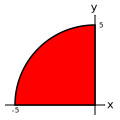
\includegraphics[width = 0.5\textwidth]{Polar_region_7}
}
\end{tabular}

The integrand is:
\[\sqrt{x^2 + y^2} = \sqrt{r^2} = r\]
so
\[\iint_R \sqrt{x^2 + y^2} \cdot dA = \iint_R r \cdot dA\]

Now to rewrite \(R\) using polar coordinates. 

The positive \(y\) and negative \(x\) axes form the lower and upper bounds on \(\theta\) whcih are \(\frac{\pi}{2}\) and \(\pi\).

The equation of the circle (which forms the upper bound on \(r\)) is:
\begin{align*}
& x = -\sqrt{25 - y^2}   
\implies r\cos\theta = -\sqrt{25 - (r\sin\theta)^2}    
\iff r^2 \cos^2\theta = 25 - r^2 \sin^2\theta \\ 
& \iff r^2 = 25 
\iff r = 5 
\end{align*}     

From the sketch, the bounds on \(\theta\) are \(\frac{\pi}{2}\) and \(\pi\), while the bounds on \(r\) are \(0\) and \(5\):
\[R = \left\{(r,\theta)\middle| \frac{\pi}{2} \leq \theta \leq \pi \;\&\; 0 \leq r \leq 5 \right\}\]

The double integral becomes the following polar nested integral. Note the inclusion of an additional factor of \(r\) in the integrand of the nested integral.
\begin{align*}
\iint_R r \cdot dA = & \int_{\theta = \pi/2}^{\pi} \left(\int_{r = 0}^{5} r^2 \cdot dr\right)d\theta 
\end{align*}
The Cartesian nested integral has been rewritten as a polar nested integral. This integral can in fact be further evaluated:

\begin{align*}
& \int_{\theta = \pi/2}^{\pi} \left(\int_{r = 0}^{5} r^2 \cdot dr\right)d\theta 
= \int_{\theta = \pi/2}^{\pi} \frac{1}{3}r^3\Big|_{r = 0}^{5} d\theta  
= \int_{\theta = \pi/2}^{\pi} \frac{125}{3} d\theta   
= \frac{125 \pi}{6}
\end{align*}

Therefore:
\[\int_{y = 0}^5 \left(\int_{x = -\sqrt{25 - y^2}}^{0} \sqrt{x^2 + y^2} dx\right)dy = \frac{125 \pi}{6}\]




\vspace{5mm}

\textbf{Example 2:}

\begin{tabular}{cc}
\parbox{0.5\textwidth}{
Consider the Cartesian nested integral:
\[\int_{x = 0}^3 \left(\int_{y = x^2}^{3x} \frac{x^4}{(x^2 + y^2)^2} dy\right)dx\] 
This integral is difficult to evaluate, and so it will be converted to polar coordinates. 
\[\int_{x = 0}^3 \left(\int_{y = x^2}^{3x} \frac{x^4}{(x^2 + y^2)^2} dy\right)dx = \iint_R \frac{x^4}{(x^2 + y^2)^2} dA\] 
where 
\[R = \{(x,y)| 0 \leq x \leq 3 \;\&\; x^2 \leq y \leq 3x\}\]
This region is sketched on the right.
} & \parbox{0.5\textwidth}{

\includegraphics[width = 0.5\textwidth]{Polar_region_3}
}
\end{tabular}

The integrand is:
\[\frac{x^4}{(x^2 + y^2)^2} 
= \frac{(r\cos\theta)^4}{(r^2)^2}
= \frac{r^4 \cos^4\theta}{r^4}
= \cos^4\theta\]
so
\[\iint_R \frac{x^4}{(x^2 + y^2)^2} dA = \iint_R \cos^4\theta dA\]

Now to rewrite \(R\) using polar coordinates. 

The line \(y = 3x\) corresponds to an upper bound of \(\theta = \tan^{-1}(3)\). 

The equation of the parabola (which forms the upper bound on \(r\)) is:
\begin{align*}
& y = x^2   
\iff r\sin\theta = (r\cos\theta)^2 
\iff r\sin\theta = r^2\cos^2\theta 
\iff (\cos^2\theta)r = \sin\theta 
\iff r = \frac{\sin\theta}{\cos^2\theta}
\end{align*}     

The parabola is tangent to the \(x\)-axis, so the lower bound on \(\theta\) is \(0\).

From the sketch, the bounds on \(\theta\) are \(0\) and \(\tan^{-1}(3)\), while the bounds on \(r\) are \(0\) and \(\frac{\sin\theta}{\cos^2\theta}\):
\[R = \left\{(r,\theta)\middle| 0 \leq \theta \leq \tan^{-1}(3) \;\&\; 0 \leq r \leq \frac{\sin\theta}{\cos^2\theta}\right\}\]

The double integral becomes the following polar nested integral. Note the inclusion of an additional factor of \(r\) in the integrand of the nested integral.
\[\iint_R \cos^4\theta dA = \int_{\theta = 0}^{\tan^{-1}(3)} \left(\int_{r = 0}^{\frac{\sin\theta}{\cos^2\theta}} \cos^4\theta \cdot r \cdot dr\right)d\theta\]
The Cartesian nested integral has been rewritten as a polar nested integral. This integral can in fact be further evaluated:

\begin{align*}
& \int_{\theta = 0}^{\tan^{-1}(3)} \left(\int_{r = 0}^{\frac{\sin\theta}{\cos^2\theta}} \cos^4\theta \cdot r \cdot dr\right)d\theta  
= \int_{\theta = 0}^{\tan^{-1}(3)} \frac{1}{2}r^2\cos^4\theta \Big|_{r = 0}^{\frac{\sin\theta}{\cos^2\theta}}d\theta \\
& = \int_{\theta = 0}^{\tan^{-1}(3)} \frac{1}{2}\sin^2\theta d\theta 
= \int_{\theta = 0}^{\tan^{-1}(3)} \frac{1 - \cos(2\theta)}{4} d\theta 
= \frac{\theta - \frac{1}{2}\sin(2\theta)}{4}\Big|_{\theta = 0}^{\tan^{-1}(3)} \\
& = \frac{1}{4}\tan^{-1}(3) - \frac{1}{8}\sin(2\tan^{-1}(3)) 
= \frac{1}{4}\tan^{-1}(3) - \frac{1}{4}\sin(\tan^{-1}(3))\cos(\tan^{-1}(3)) \\
& = \frac{1}{4}\tan^{-1}(3) - \frac{1}{4}\frac{3}{\sqrt{10}}\frac{1}{\sqrt{10}} 
= \frac{1}{4}\tan^{-1}(3) - \frac{3}{40} 
\end{align*}

Therefore:
\[\int_{x = 0}^3 \left(\int_{y = x^2}^{3x} \frac{x^4}{(x^2 + y^2)^2} dy\right)dx = \frac{1}{4}\tan^{-1}(3) - \frac{3}{40}\]




\vspace{5mm}

\textbf{Example 3:}

\begin{tabular}{cc}
\parbox{0.5\textwidth}{
Consider the Cartesian nested integral:
\[\int_{x = 0}^3 \left(\int_{y = 0}^{4 - \frac{4}{3}x} \frac{4x + 3y}{x^2 + y^2} dy\right)dx\] 
This integral is difficult to evaluate, and so it will be converted to polar coordinates. 
\[\int_{x = 0}^3 \left(\int_{y = 0}^{4 - \frac{4}{3}x} \frac{4x + 3y}{x^2 + y^2} dy\right)dx = \iint_R \frac{4x + 3y}{x^2 + y^2} dA\] 
where 
\[R = \{(x,y)| 0 \leq x \leq 3 \;\&\; 0 \leq y \leq 4 - \frac{4}{3}x\}\]
This region is sketched on the right.
} & \parbox{0.5\textwidth}{

\includegraphics[width = 0.5\textwidth]{Polar_region_4}
}
\end{tabular}

The integrand is:
\[\frac{4x + 3y}{x^2 + y^2} 
= \frac{4r\cos\theta + 3r\sin\theta}{r^2}
= \frac{4\cos\theta + 3\sin\theta}{r}\]
so
\[\iint_R \frac{4x + 3y}{x^2 + y^2} dA = \iint_R \frac{4\cos\theta + 3\sin\theta}{r} dA\]

Now to rewrite \(R\) using polar coordinates. 

The positive \(x\) and positive \(y\) axes form the lower and upper bounds on \(\theta\) whcih are \(0\) and \(\frac{\pi}{2}\).

The equation of the line (which forms the upper bound on \(r\)) is:
\begin{align*}
& y = 4 - \frac{4}{3}x   
\iff r\sin\theta = 4 - \frac{4}{3}r\cos\theta 
\iff (\frac{4}{3}\cos\theta + \sin\theta)r = 4 
\iff r = \frac{12}{4\cos\theta + 3\sin\theta} 
\end{align*}     

From the sketch, the bounds on \(\theta\) are \(0\) and \(\frac{\pi}{2}\), while the bounds on \(r\) are \(0\) and \(\frac{12}{4\cos\theta + 3\sin\theta}\):
\[R = \left\{(r,\theta)\middle| 0 \leq \theta \leq \frac{\pi}{2} \;\&\; 0 \leq r \leq \frac{12}{4\cos\theta + 3\sin\theta}\right\}\]

The double integral becomes the following polar nested integral. Note the inclusion of an additional factor of \(r\) in the integrand of the nested integral.
\begin{align*}
\iint_R \frac{4\cos\theta + 3\sin\theta}{r} dA = & \int_{\theta = 0}^{\pi/2} \left(\int_{r = 0}^{\frac{12}{4\cos\theta + 3\sin\theta}} \frac{4\cos\theta + 3\sin\theta}{r} \cdot r \cdot dr\right)d\theta \\
= & \int_{\theta = 0}^{\pi/2} \left(\int_{r = 0}^{\frac{12}{4\cos\theta + 3\sin\theta}} (4\cos\theta + 3\sin\theta)dr\right)d\theta
\end{align*}
The Cartesian nested integral has been rewritten as a polar nested integral. This integral can in fact be further evaluated:

\begin{align*}
& \int_{\theta = 0}^{\pi/2} \left(\int_{r = 0}^{\frac{12}{4\cos\theta + 3\sin\theta}} (4\cos\theta + 3\sin\theta)dr\right)d\theta 
= \int_{\theta = 0}^{\pi/2} (4\cos\theta + 3\sin\theta)r \Big|_{r = 0}^{\frac{12}{4\cos\theta + 3\sin\theta}} d\theta \\ 
& = \int_{\theta = 0}^{\pi/2} 12 d\theta 
= 12\theta \Big|_{\theta = 0}^{\pi/2} 
= 6\pi
\end{align*}

Therefore:
\[\int_{x = 0}^3 \left(\int_{y = 0}^{4 - \frac{4}{3}x} \frac{4x + 3y}{x^2 + y^2} dy\right)dx = 6\pi\]





\vspace{5mm}

\textbf{Example 4:}

\vspace{5mm}

\begin{tabular}{cc}
\parbox{0.5\textwidth}{
Those familiar with probability theory will have been introduced to the ``normal" probability distribution:
\[\Pr(x) = \frac{1}{\sqrt{2\pi}}e^{-\frac{1}{2}x^2}\]
This probability distribution is a ``bell curve" where the variance is \(1\).

The natural question if where does the coefficient of \(\frac{1}{\sqrt{2\pi}}\) come from? The answer is that the coefficient makes the total probability equal to 1:
\[\int_{x = -\infty}^{+\infty} \Pr(x) dx = 1\]
} & \parbox{0.5\textwidth}{
\includegraphics[width = 0.5\textwidth]{bell_curve_plot.png}
}
\end{tabular}

This means that 
\[\int_{x = -\infty}^{+\infty} e^{-\frac{1}{2}x^2} dx = \sqrt{2\pi}\]
{\bf How can this be proven?} An anti-derivative for the function \(e^{-\frac{1}{2}x^2}\) cannot be expressed in terms of the ``usual" mathematical symbols \(+\), \(-\), \(\times\), \(\div\), \(\exp\), \(\log\), \(\cos\), \(\sin\), etc. Despite this, the definite integral \(\int_{x = -\infty}^{+\infty} e^{-\frac{1}{2}x^2} dx\) can still be computed. 

Let \(I = \int_{x = -\infty}^{+\infty} e^{-\frac{1}{2}x^2} dx\), so 
\begin{align*}
I^2 = & \left(\int_{x = -\infty}^{+\infty} e^{-\frac{1}{2}x^2} dx\right)^2 \\
= & \left(\int_{x = -\infty}^{+\infty} e^{-\frac{1}{2}x^2} dx\right)\left(\int_{x = -\infty}^{+\infty} e^{-\frac{1}{2}x^2} dx\right)
= \left(\int_{x = -\infty}^{+\infty} e^{-\frac{1}{2}x^2} dx\right)\left(\int_{y = -\infty}^{+\infty} e^{-\frac{1}{2}y^2} dy\right) \\ 
= & \int_{x = -\infty}^{+\infty} e^{-\frac{1}{2}x^2}\left(\int_{y = -\infty}^{+\infty} e^{-\frac{1}{2}y^2} dy\right) dx 
= \int_{x = -\infty}^{+\infty} \left(\int_{y = -\infty}^{+\infty} e^{-\frac{1}{2}x^2}e^{-\frac{1}{2}y^2} dy\right) dx \\ 
= & \int_{x = -\infty}^{+\infty} \left(\int_{y = -\infty}^{+\infty} e^{-\frac{1}{2}(x^2 + y^2)} dy\right) dx
\end{align*}

This Cartesian nested integral will be evaluated by converting it to a polar nested integral.
\[\int_{x = -\infty}^{+\infty} \left(\int_{y = -\infty}^{+\infty} e^{-\frac{1}{2}(x^2 + y^2)} dy\right) dx = \iint_R e^{-\frac{1}{2}(x^2 + y^2)}dA\]
where \(R\) is the set of all points in 2D space:
\[R = \{(x,y) | -\infty < x < +\infty \;\&\; -\infty < y < +\infty\}\]

The integrand is:
\[e^{-\frac{1}{2}(x^2 + y^2)} = e^{-\frac{1}{2}r^2}\]
so
\[\iint_R e^{-\frac{1}{2}(x^2 + y^2)}dA = \iint_R e^{-\frac{1}{2}r^2}dA\]

In terms of polar coordinates, the set of points in 2D space can be expressed as:
\[R = \{(r,\theta) | 0 \leq r \leq +\infty \;\&\; 0 \leq \theta \leq 2\pi \}\]

The double integral becomes the following polar nested integral. Note the inclusion of an additional factor of \(r\) in the integrand of the nested integral.
\begin{align*}
\iint_R e^{-\frac{1}{2}r^2}dA = & \int_{\theta = 0}^{2\pi} \left(\int_{r = 0}^{+\infty} e^{-\frac{1}{2}r^2} \cdot r \cdot dr \right)d\theta
\end{align*}
The Cartesian nested integral has been rewritten as a polar nested integral. {\bf The additional factor of \(r\) in the integrand is what makes this integral solvable using the chain rule.} This integral can in fact be further evaluated:

\begin{align*}
& \int_{\theta = 0}^{2\pi} \left(\int_{r = 0}^{+\infty} e^{-\frac{1}{2}r^2} \cdot r \cdot dr \right)d\theta 
= \int_{\theta = 0}^{2\pi} -e^{-\frac{1}{2}r^2}\Big|_{r = 0}^{+\infty} d\theta 
= \int_{\theta = 0}^{2\pi} (0 - (-1))d\theta 
= \int_{\theta = 0}^{2\pi} d\theta 
= \theta\Big|_{\theta = 0}^{2\pi}
= 2\pi
\end{align*}
Therefore \(I^2 = 2\pi\), so \(I = \sqrt{2\pi}\). Therefore:
\[\int_{x = -\infty}^{+\infty} e^{-\frac{1}{2}x^2} dx = \sqrt{2\pi}\]
This explains why the normal distribution has the coefficient \(\frac{1}{\sqrt{2\pi}}\). 




\section*{Polar integral to Cartesian integral conversions} 

Often, it may be necessary to convert a nested integral that uses polar coordinates to a nested integral that uses Cartesian coordinates. Firstly, the nested polar integral needs to be converted to a double integral. The limits of integration define the region of integration for the double integral:

\[\int_{\theta = a}^b \left(\int_{r = h_L(\theta)}^{h_U(\theta)} f(r,\theta)dr\right)d\theta = \iint_R \frac{f(r,\theta)}{r}dA \quad\text{where}\quad R = \{(r,\theta) | a \leq \theta \leq b \;\&\; h_L(\theta) \leq r \leq h_U(\theta)\}\] 

When the polar nested integral is converted to a double integral, the integrand is divided by \(r\) to remove the factor of \(r\) that is present in the polar nested integral. 

Once the nested integral has been converted to a double integral, the integrand needs to be rewritten to use Carteisan coordinates \(x\) and \(y\) instead of \(r\) and \(\theta\). This is done using the following replacements:
\begin{itemize}
\item Replace \(\cos\theta\) with \(x/r\)
\item Replace \(\sin\theta\) with \(y/r\)
\item Replace \(\tan\theta\) with \(y/x\)
\item Replace \(\sec\theta\) with \(r/x\)
\item Replace \(\cot\theta\) with \(x/y\)
\item Replace \(\csc\theta\) with \(r/y\)
\end{itemize}
Next, the expression should be simplified to eliminate as many instances of \(r\) as possible. After as many instances of \(r\) have been eliminated, the remaining appearances of \(r\) should be replaced.
\begin{itemize}
\item Replace \(r\) with \(\sqrt{x^2 + y^2}\) 
\end{itemize} 
\textbf{Examples:}
\begin{itemize}
%\item
%\[\iint_R \tan\theta dA = \iint_R \frac{\sin\theta}{\cos\theta} dA = \iint_R \frac{y/r}{x/r} dA = \iint_R \frac{y}{x} dA\]
\item
\[\iint_R r\sec\theta dA = \iint_R r \cdot \frac{r}{x} dA = \iint_R \frac{r^2}{x} dA = \iint_R \frac{x^2 + y^2}{x} dA\]
\item
\[\iint_R r^3\cos\theta dA = \iint_R r^3(x/r)dA = \iint_R r^2 x dA = \iint_R (x^2 + y^2) x dA\]
\item
\[\iint_R r^2\cos\theta\sin\theta dA = \iint_R r^2(x/r)(y/r)dA = \iint_R xy dA\]
\end{itemize}
The region \(R\) needs to be expressed using Cartesian coordinates. The first thing to do is to {\bf sketch the region} \(R\). The sketch will help keep track of which curves/lines form which limits and boundaries. The equations for the curves that bound \(R\) need to have \(r\) and \(\theta\) replaced so the equation now uses Carteisan coordinates. The equation is then rewritten so \(y\) is a function of \(x\), or \(x\) is a constant value (or express \(x\) as a function of \(y\)). When simplifying the equation, the case where \(r = 0\) can often be simply ignored so division of both sides by \(r\) can be done safely.

In particular, the bounds on \(\theta\) correspond to straight lines that pass through the origin. The condition \(\theta = a\) corresponds to the line \(y = \tan(a) x\). 

Lastly, the double integral is converted to a Cartesian nested integral.





\vspace{5mm}

\textbf{Example 1:}

\vspace{5mm}

\begin{tabular}{cc}
\parbox{0.5\textwidth}{
Consider the polar nested integral:
\[\int_{\theta = 0}^{\pi} \left(\int_{r = 0}^{5} \frac{r}{\sqrt{25 - r^2\cos^2\theta}} dr\right)d\theta\] 
This integral is difficult to evaluate, and so it will be converted to Cartesian coordinates. 
\begin{align*}
& \int_{\theta = 0}^{\pi} \left(\int_{r = 0}^{5} \frac{r}{\sqrt{25 - r^2\cos^2\theta}} dr\right)d\theta \\
& = \iint_R \frac{1}{\sqrt{25 - r^2\cos^2\theta}} dA
\end{align*} 
where 
\[R = \Big\{(r,\theta) \Big| 0 \leq \theta \leq \pi \;\&\; 0 \leq r \leq 5\Big\}\]   
This region is sketched on the right. 

Note the removal of a factor of \(r\) from the integrand.
} & \parbox{0.5\textwidth}{
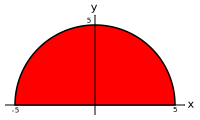
\includegraphics[width = 0.5\textwidth]{Polar_region_8}
}
\end{tabular}

\vspace{5mm}

The integrand is:
\[\frac{1}{\sqrt{25 - r^2\cos^2\theta}} = \frac{1}{\sqrt{25 - r^2(x/r)^2}} = \frac{1}{\sqrt{25 - x^2}}\]
so
\[\iint_R \frac{1}{\sqrt{25 - r^2\cos^2\theta}} dA = \iint_R \frac{1}{\sqrt{25 - x^2}} dA\]

Now to rewrite \(R\) using Carteisan coordinates. 

The bounds on \(x\) are \(-5\) and \(5\). The lower bound on \(y\) is \(0\). The curve \(r = 5\) defines the upper bound on \(y\):
\begin{align*}
& r = 5 
\iff \sqrt{x^2 + y^2} = 5 
\iff x^2 + y^2 = 25 
\iff y^2 = 25 - x^2 
\iff y = \pm\sqrt{25 - x^2}
\end{align*}
The upper bound on \(y\) is the non-negative solution, \(\sqrt{25 - x^2}\).

\[R = \{(x,y) | -5 \leq x \leq 5 \;\&\; 0 \leq y \leq \sqrt{25 - x^2}\}\] 

The double integral becomes the following Cartesian nested integral. 
\[\iint_R \frac{1}{\sqrt{25 - x^2}} dA = \int_{x = -5}^{5} \left(\int_{y = 0}^{\sqrt{25 - x^2}} \frac{1}{\sqrt{25 - x^2}} dy\right)dx\]
The polar nested integral has been rewritten as a Carteisan nested integral. This integral can in fact be further evaluated:

\begin{align*}
& \int_{x = -5}^{5} \left(\int_{y = 0}^{\sqrt{25 - x^2}} \frac{1}{\sqrt{25 - x^2}} dy\right)dx 
= \int_{x = -5}^{5} \frac{y}{\sqrt{25 - x^2}}\Big|_{y = 0}^{\sqrt{25 - x^2}} dx 
= \int_{x = -5}^{5} dx 
= x\Big|_{x = -5}^{5}
= 10
\end{align*}

Therefore:
\[\int_{\theta = 0}^{\pi} \left(\int_{r = 0}^{5} \frac{r}{\sqrt{25 - r^2\cos^2\theta}} dr\right)d\theta = 10\] 





\vspace{5mm}

\textbf{Example 2:}

\vspace{5mm}

\begin{tabular}{cc}
\parbox{0.5\textwidth}{
Consider the polar nested integral:
\[\int_{\theta = 0}^{\pi/2} \left(\int_{r = 0}^{\frac{12}{4\cos\theta + 3\sin\theta}} r^2\cos\theta dr\right)d\theta\] 
This integral is difficult to evaluate, and so it will be converted to Cartesian coordinates. 
\[\int_{\theta = 0}^{\pi/2} \left(\int_{r = 0}^{\frac{12}{4\cos\theta + 3\sin\theta}} r^2\cos\theta dr\right)d\theta = \iint_R r\cos\theta dA\] 
where 
\[R = \left\{(r,\theta) \middle| 0 \leq \theta \leq \frac{\pi}{2} \;\&\; 0 \leq r \leq \frac{12}{4\cos\theta + 3\sin\theta} \right\}\]
This region is sketched on the right. 

Note the removal of a factor of \(r\) from the integrand.
} & \parbox{0.5\textwidth}{

\includegraphics[width = 0.5\textwidth]{Polar_region_5}
}
\end{tabular}

The integrand is:
\[r\cos\theta = r(x/r) = x\]
so
\[\iint_R r\cos\theta dA = \iint_R x dA\]

Now to rewrite \(R\) using Carteisan coordinates. 

The lower bound on \(\theta\), \(\theta = 0\), is the positive \(x\)-axis. 

The upper bound on \(\theta\), \(\theta = \frac{\pi}{2}\), is the positive \(y\)-axis. 

The equation of the curve \(r = \frac{12}{4\cos\theta + 3\sin\theta}\) (which forms the upper bound on \(y\)) is: 
\begin{align*}
& r = \frac{12}{4\cos\theta + 3\sin\theta} 
\iff r = \frac{12}{4(x/r) + 3(y/r)}    
\iff r = \frac{12r}{4x + 3y} 
\iff 1 = \frac{12}{4x + 3y} \\
& \iff 4x + 3y = 12 
\iff y = 4 - \frac{4}{3}x
\end{align*}

From the sketch, the bounds on \(x\) are \(0\) and \(3\), while the bounds on \(y\) are \(0\) and \(4 - \frac{4}{3}x\):
\[R = \left\{(x, y)\middle| 0 \leq x \leq 3 \;\&\; 0 \leq y \leq 4 - \frac{4}{3}x\right\}\]

The double integral becomes the following Cartesian nested integral. 
\[\iint_R x dA = \int_{x = 0}^{3} \left(\int_{y = 0}^{4 - \frac{4}{3}x} x dy\right)dx\]
The polar nested integral has been rewritten as a Carteisan nested integral. This integral can in fact be further evaluated:

\begin{align*}
& \int_{x = 0}^{3} \left(\int_{y = 0}^{4 - \frac{4}{3}x} x dy\right)dx 
= \int_{x = 0}^{3} xy\Big|_{y = 0}^{4 - \frac{4}{3}x} dx 
= \int_{x = 0}^{3} (4x - \frac{4}{3}x^2) dx 
= (2x^2 - \frac{4}{9}x^3)\Big|_{x = 0}^{3} \\
& = (18 - 12) - 0 
= 6 
\end{align*}

Therefore:
\[\int_{\theta = 0}^{\pi/2} \left(\int_{r = 0}^{\frac{12}{4\cos\theta + 3\sin\theta}} r^2\cos\theta dr\right)d\theta = 6\]





\vspace{5mm}

\textbf{Example 3:}

\vspace{5mm}

\begin{tabular}{cc}
\parbox{0.5\textwidth}{
Consider the polar nested integral:
\[\int_{\theta = \tan^{-1}(2/5)}^{\tan^{-1}(7/5)} \left(\int_{r = \sec\theta}^{5\sec\theta} \frac{r}{(r\sin\theta - \frac{2}{5}r\cos\theta + 1)^2} dr\right)d\theta\] 
This integral is difficult to evaluate, and so it will be converted to Cartesian coordinates. 
\begin{align*}
& \int_{\theta = \tan^{-1}(2/5)}^{\tan^{-1}(7/5)} \left(\int_{r = \sec\theta}^{5\sec\theta} \frac{r}{(r\sin\theta - \frac{2}{5}r\cos\theta + 1)^2} dr\right)d\theta \\
& = \iint_R \frac{1}{(r\sin\theta - \frac{2}{5}r\cos\theta + 1)^2} dA
\end{align*} 
where 
\begin{align*}  
R = & \Big\{(r,\theta) \Big| \tan^{-1}(2/5) \leq \theta \leq \tan^{-1}(7/5) \\
& \quad\quad\quad\;\&\; \sec\theta \leq r \leq 5\sec\theta \Big\}
\end{align*}  
This region is sketched on the right. 

Note the removal of a factor of \(r\) from the integrand.
} & \parbox{0.5\textwidth}{

\includegraphics[width = 0.5\textwidth]{Polar_region_6}
}
\end{tabular}

The integrand is:
\[\frac{1}{(r\sin\theta - \frac{2}{5}r\cos\theta + 1)^2} = \frac{1}{(r(y/r) - \frac{2}{5}r(x/r) + 1)^2} = \frac{1}{(y - \frac{2}{5}x + 1)^2}\]
so
\[\iint_R \frac{1}{(r\sin\theta - \frac{2}{5}r\cos\theta + 1)^2} dA = \iint_R \frac{1}{(y - \frac{2}{5}x + 1)^2} dA\]

Now to rewrite \(R\) using Carteisan coordinates. 

The lower bound on \(\theta\), \(\theta = \tan^{-1}(2/5)\), is the line \(y = \frac{2}{5}x\). 

The upper bound on \(\theta\), \(\theta = \tan^{-1}(7/5)\), is the line \(y = \frac{7}{5}x\). 

The equation of the curve \(r = \sec\theta\) is: 
\begin{align*}
& r = \sec\theta 
\iff r = \frac{1}{\cos\theta}    
\iff r = \frac{1}{x/r} 
\iff r = \frac{r}{x} 
\iff 1 = \frac{1}{x} 
\iff x = 1
\end{align*}

The equation of the curve \(r = 5\sec\theta\) is: 
\begin{align*}
& r = 5\sec\theta 
\iff r = \frac{5}{\cos\theta}    
\iff r = \frac{5}{x/r} 
\iff r = \frac{5r}{x} 
\iff 1 = \frac{5}{x} 
\iff x = 5
\end{align*}

From the sketch, the bounds on \(x\) are \(1\) and \(5\), while the bounds on \(y\) are \(\frac{2}{5}x\) and \(\frac{7}{5}x\):
\[R = \left\{(x, y)\middle| 1 \leq x \leq 5 \;\&\; \frac{2}{5}x \leq y \leq \frac{7}{5}x\right\}\]

The double integral becomes the following Cartesian nested integral. 
\[\iint_R \frac{1}{(y - \frac{2}{5}x + 1)^2} dA = \int_{x = 1}^{5} \left(\int_{y = (2/5)x}^{(7/5)x} \frac{1}{(y - \frac{2}{5}x + 1)^2} dy\right)dx\]
The polar nested integral has been rewritten as a Carteisan nested integral. This integral can in fact be further evaluated:

\begin{align*}
& \int_{x = 1}^{5} \left(\int_{y = (2/5)x}^{(7/5)x} \frac{1}{(y - \frac{2}{5}x + 1)^2} dy\right)dx 
= \int_{x = 1}^{5} \frac{-1}{y - \frac{2}{5}x + 1}\Big|_{y = (2/5)x}^{(7/5)x} dx   
= \int_{x = 1}^{5} \left(\frac{-1}{x + 1} - (-1)\right) dx \\  
& = \int_{x = 1}^{5} \left(1 - \frac{1}{x + 1}\right) dx 
= (x - \ln|x + 1|)\Big|_{x = 1}^{5} 
= (5 - \ln(6)) - (1 - \ln(2)) 
= 4 - \ln(3)
\end{align*}

Therefore:
\[\int_{\theta = \tan^{-1}(2/5)}^{\tan^{-1}(7/5)} \left(\int_{r = \sec\theta}^{5\sec\theta} \frac{r}{(r\sin\theta - \frac{2}{5}r\cos\theta + 1)^2} dr\right)d\theta = 4 - \ln(3)\]




\end{document}

















